%% Primeira versão completa. Modelo Springer Nature (sn-jnl), estilo de
%% referências autor-ano (sn-basic), como pedem as instruções da DMKD.
%% As tabelas em tables/ são geradas por make_tables.py a partir dos CSVs
%% de resultados; não editar à mão.
\documentclass[pdflatex,sn-basic]{sn-jnl}

\usepackage[T1]{fontenc}
\usepackage{lmodern}
\usepackage{graphicx}
\usepackage{multirow}
\usepackage{amsmath,amssymb,amsfonts}
\usepackage{amsthm}
\usepackage[title]{appendix}
\usepackage{xcolor}
\usepackage{booktabs}
\usepackage{manyfoot}
\usepackage{algorithm}
\usepackage{algorithmicx}
\usepackage{algpseudocode}
\usepackage{tikz}
\usetikzlibrary{arrows.meta,positioning,fit,backgrounds}

\newcommand{\DL}{\mathcal{D}_L}
\newcommand{\DU}{\mathcal{D}_U}
\newcommand{\Cold}{\mathcal{C}_{\mathrm{old}}}
\newcommand{\Cnew}{\mathcal{C}_{\mathrm{new}}}
\newcommand{\todo}[1]{\textcolor{red}{[#1]}}

\raggedbottom

\begin{document}

\title[One-class decomposition for category discovery in tabular data]{Reject, then discover: one-class decomposition with conformal rejection for generalized and incremental category discovery in tabular data}

\author*[1]{\fnm{Luiz S.} \sur{Oliveira}}\email{\todo{e-mail}}
\author[2]{\fnm{George D. C.} \sur{Cavalcanti}}\email{\todo{e-mail}}

\affil*[1]{\orgdiv{Departamento de Inform\'atica}, \orgname{Universidade Federal do Paran\'a (UFPR)}, \orgaddress{\city{Curitiba}, \state{PR}, \country{Brazil}}}
\affil[2]{\orgdiv{Centro de Inform\'atica}, \orgname{Universidade Federal de Pernambuco (UFPE)}, \orgaddress{\city{Recife}, \state{PE}, \country{Brazil}}}

\abstract{Generalized category discovery asks a model to label an unlabeled set that mixes samples of known classes with samples of classes never seen during training. Most methods learn a representation per problem with deep networks, and tabular methods assume that the unlabeled set holds only novel classes. We study the problem with fixed representations and modest computing resources, and decompose it into one one-class classifier per known class, trained only on labeled data. Conformal calibration places the classifiers on a common scale, a sample that every classifier rejects becomes a candidate novelty, and the rejected set is clustered by a density-based procedure whose minimum cluster size is derived from the expected number of samples of known classes rejected by mistake. The family of one-class classifier is chosen per data set by hiding known classes, without looking at the unlabeled data. Since adding a class only adds a classifier, the model also handles incremental sessions without storing past data. On 15 tabular data sets, the approach has the best mean rank in the transductive setting and significantly outperforms the clustering baselines, while its advantage over a random forest with maximum softmax rejection and over PBN, a recent method for tabular novel class discovery, is consistent but not significant. In the incremental setting it matches a random forest retrained at every session without storing data. In the four data sets where no method separates novel from known samples, a random forest trained with all labels also reaches at most 0.66 accuracy.}

\keywords{Generalized category discovery, Novel class discovery, One-class classification, Conformal prediction, Tabular data, Incremental learning}

\maketitle

%% ===================================================================
\section{Introduction}\label{sec:intro}

A classifier deployed in an open world eventually receives samples of classes that did not exist when it was trained. Novel class discovery (NCD) and its generalization, generalized category discovery (GCD), turn this situation into a learning problem: given a labeled set $\DL$ with samples of known classes and an unlabeled set $\DU$, assign a label to every sample of $\DU$, either one of the known classes or one of the novel classes, which must be discovered \citep{hsu2018kcl,han2019dtc,vaze2022gcd}. In NCD the unlabeled set contains only novel classes; in GCD it mixes known and novel classes, which is the more realistic case and the one we address.

Most of the literature comes from computer vision, where the representation is learned or fine-tuned for each problem with self-supervised and supervised objectives on large networks \citep{fini2021uno,vaze2022gcd,wen2023simgcd}. Tabular data received much less attention. TabularNCD \citep{troisemaine2022tabularncd} and PBN \citep{troisemaine2024pbn} adapted the NCD recipe to tabular data by training a projection network on the known classes and clustering the novel samples in the learned space. The authors of PBN also insisted that hyperparameters be chosen without the labels of the novel classes, a constraint we adopt. Both methods assume the NCD setting, in which every unlabeled sample is novel, and both must be retrained when new classes arrive.

Tabular data has two features that motivate a different design. First, tree ensembles on the original attributes remain hard to beat \citep{grinsztajn2022tabular}, so a learned representation is not a given. Second, many tabular applications must update the model with modest computing resources, often without a GPU and without keeping the raw data. We therefore ask how far one can go in GCD with a fixed representation, using models that train in seconds on a CPU.

Our answer is to reject before discovering. We decompose the multi-class problem into one one-class classifier (OCC) per known class \citep{tax2004svdd,khan2014occ}, trained only on $\DL$. A sample that every OCC rejects is a candidate novelty; the rest keep the label of the class that accepts them.

Each OCC outputs a raw score whose scale depends on the family and on the class. We convert the scores into conformal p-values \citep{vovk2005alrw,bates2023conformal}, which puts all classes on the same scale and turns the rejection threshold into a parameter $\alpha$ with a direct reading: the fraction of samples of a known class expected to be rejected by mistake.

Those samples are the main obstacle to discovery. They form small groups in the rejected set, and a clustering algorithm reports them as novel classes. Since the calibration tells us how many to expect, we use that number as the minimum cluster size of HDBSCAN \citep{campello2013hdbscan}, and fragments of known classes stop becoming classes.

No OCC family is best on every data set. We pick the family for each data set by hiding known classes in $\DL$ and measuring how well each family rejects them, the same device that \citet{troisemaine2024pbn} use to tune PBN.

The decomposition has a structural advantage for incremental discovery. Adding a class means adding an OCC; the existing classifiers are not retrained, and no sample of past sessions needs to be stored. We exploit this in an incremental setting where novel classes arrive in a stream of unlabeled sessions.

This work continues our research on one-class decomposition for multi-class problems \citep{fragoso2021modes} and on open set recognition in dissimilarity spaces \citep{teixeira2025osr}, and extends it from closed-set classification and rejection to discovery. Our contributions are:

\begin{enumerate}
\item A GCD method for fixed representations based on one calibrated OCC per class, a discovery step whose minimum cluster size comes from the expected number of rejected known samples, and a family selection procedure that uses only labeled data (Sect.~\ref{sec:method}).
\item An incremental variant that incorporates discovered classes without retraining or storing data (Sect.~\ref{sec:incremental}).
\item An evaluation on 15 tabular data sets, the seven used by PBN and eight selected from OpenML by criteria fixed in advance, in the transductive and incremental settings, against clustering baselines, closed-set classifiers with maximum softmax probability rejection and PBN, which we reimplemented and validated against its published results (Sects.~\ref{sec:protocol} and \ref{sec:results}).
\item An analysis of when discovery is possible at all: in four data sets no method separates novel from known samples, and a supervised classifier trained with all labels also performs poorly there, so the difficulty lies in the data (Sect.~\ref{sec:detectability}).
\end{enumerate}

In the transductive setting the method has the best mean rank and outperforms the clustering baselines with statistical significance, but its advantage over the random forest with softmax rejection and over PBN is not significant across 15 data sets. In the incremental setting it matches a random forest that is retrained at every session and keeps all past data, while it stores none.

%% ===================================================================
\section{Related work}\label{sec:related}

\paragraph{Novel and generalized category discovery.}
NCD was formulated as transfer of a notion of similarity from labeled to unlabeled classes \citep{hsu2018kcl} and developed with deep clustering \citep{han2019dtc} and unified objectives over labeled and unlabeled heads \citep{fini2021uno}. \citet{vaze2022gcd} introduced GCD, in which the unlabeled set mixes known and novel classes, together with a semi-supervised $k$-means baseline on a contrastively fine-tuned vision transformer; SimGCD \citep{wen2023simgcd} replaced the clustering step by a parametric classifier. These methods fine-tune large networks and are evaluated on images. Their unlabeled samples of known classes are handled implicitly by the clustering or the classifier; there is no explicit rejection step.

\paragraph{Discovery in tabular data.}
TabularNCD \citep{troisemaine2022tabularncd} brought NCD to tabular data with a network trained on known classes and pseudo-labels on the unlabeled set. PBN \citep{troisemaine2024pbn} simplified it: a projection network is trained with a classification loss on the known classes and a reconstruction loss on all data, and the novel samples are clustered with $k$-means in the latent space. The same work proposed a hyperparameter search that hides known classes, which we adopt in spirit for family selection, and estimated the number of novel classes with the silhouette in the latent space. PBN addresses NCD; we evaluate it in GCD as well, where its clustering must also absorb the unlabeled samples of known classes.

\paragraph{Incremental discovery.}
Class-incremental NCD \citep{roy2022incd,joseph2022ncdwf} and continual GCD \citep{wu2023metagcd} consider classes arriving over time and focus on avoiding catastrophic forgetting in deep networks, usually with distillation or stored prototypes. In our setting forgetting is avoided by construction, since the classifiers of past classes are never retrained.

\paragraph{One-class classification and decomposition.}
One-class classifiers model a single class and reject the rest \citep{tax2004svdd,scholkopf2001ocsvm,khan2014occ,pimentel2014novelty}. Decomposing a multi-class problem into one OCC per class gives a classifier that can reject \citep{krawczyk2016dcs}; MODES \citep{fragoso2021modes} combined such a decomposition with dynamic selection of OCCs trained on clusters of each class. Our OCC families include the minimum spanning tree data description \citep{juszczak2009mstdd} and a classifier in the dissimilarity space \citep{cha2000dichotomy,teixeira2025osr}. We use the decomposition for a different goal: the rejected samples are clustered into new classes, which are then added to the decomposition.

\paragraph{Open set recognition and conformal p-values.}
Open set recognition rejects samples of unknown classes \citep{scheirer2013osr}; the maximum softmax probability (MSP) of a closed-set classifier is a simple and competitive rejection score \citep{hendrycks2017msp}, which we use as a baseline rejector. Conformal prediction \citep{vovk2005alrw} converts any score into a p-value whose guarantee holds for finite samples under exchangeability, and \citet{bates2023conformal} studied conformal p-values as tests for outliers. We use cross-validation to compute calibration scores, as in cross-conformal prediction \citep{vovk2015crossconformal}, because known classes can be small.

%% ===================================================================
\section{Problem settings}\label{sec:settings}

Let $\Cold$ be the set of known classes and $\Cnew$ the set of novel classes, with $\Cold \cap \Cnew = \emptyset$. Samples are vectors $x \in \mathbb{R}^d$ in a fixed representation.

\paragraph{Transductive GCD (C2).} We receive $\DL = \{(x_i, y_i)\}$ with $y_i \in \Cold$ and $\DU = \{x_j\}$ whose true labels lie in $\Cold \cup \Cnew$. The task is to predict a label for every $x_j \in \DU$; predicted novel labels are arbitrary identifiers. The number of novel classes $|\Cnew|$ is either given (``$K$ known'') or must be estimated (``$K$ estimated''), the realistic case and our main setting.

\paragraph{Incremental GCD (C4).} A labeled session $S_0$ with samples of $\Cold$ is followed by $T$ unlabeled sessions $U_1, \dots, U_T$. Each session contains samples of the known classes, samples of novel classes that appear for the first time and further samples of novel classes that appeared in earlier sessions. After each session the model must label the session, and the classes it discovered must be recognized, not rediscovered, in later sessions. No labels are available after $S_0$.

\paragraph{NCD (C1).} The unlabeled set contains only novel classes. This is the setting of PBN; we use it only to validate our reimplementation of PBN (Appendix~\ref{app:pbn}).

\paragraph{Evaluation.} In C2 we report clustering accuracy under the optimal assignment of predicted to true labels, each true label receiving at most one predicted label, computed once over all of $\DU$ (Hungarian matching), and accuracies on the samples of old and new classes under that same assignment (ACC All, Old and New), following \citet{vaze2022gcd} and \citet{wen2023simgcd}. In C4 the assignment of a discovered cluster to a true class is made in the session in which the cluster appears and kept fixed afterwards, so that an error of discovery propagates to later sessions as it would in practice. We report the mean over sessions of ACC All, Old (classes seen before the session) and New (classes that debut in the session), and forgetting, the drop in accuracy on the classes of $S_0$ between the first and the last session.

%% ===================================================================
\section{Method}\label{sec:method}

Figure~\ref{fig:overview} summarizes the method. We describe the one-class decomposition and its calibration (Sect.~\ref{sec:occ}), the choice of the OCC family (Sect.~\ref{sec:selection}), the discovery step (Sect.~\ref{sec:discovery}) and the incremental variant (Sect.~\ref{sec:incremental}).

\begin{figure}[t]
\centering
\resizebox{\linewidth}{!}{%
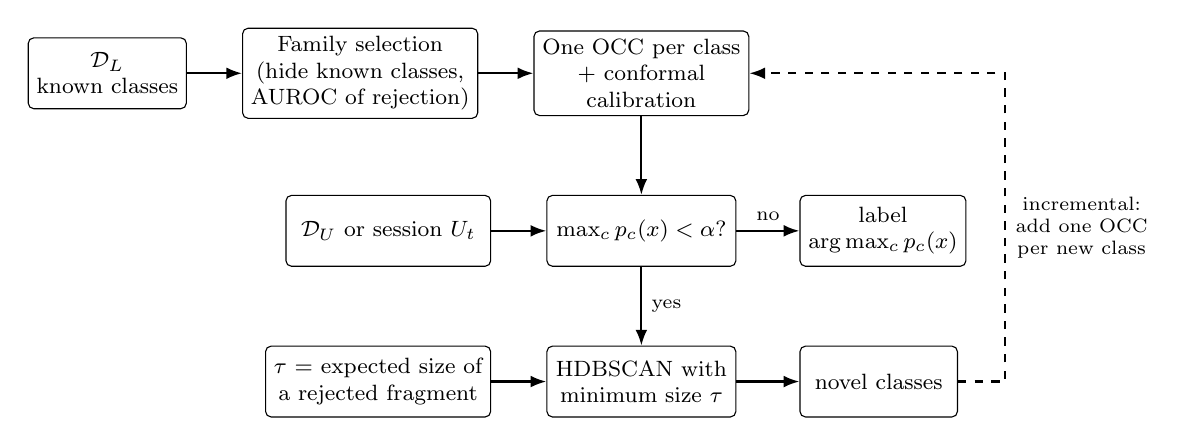
\begin{tikzpicture}[
  box/.style={draw, rounded corners=2pt, align=center, font=\footnotesize, minimum height=9mm, inner sep=3pt},
  arr/.style={-{Latex[length=2mm]}, thick},
  lab/.style={font=\scriptsize, align=center}]
\node[box, minimum width=18mm] (dl) {$\mathcal{D}_L$\\known classes};
\node[box, right=7mm of dl, minimum width=26mm] (sel) {Family selection\\(hide known classes,\\AUROC of rejection)};
\node[box, right=7mm of sel, minimum width=24mm] (occ) {One OCC per class\\+ conformal\\calibration};
\node[box, below=10mm of occ, minimum width=24mm] (rej) {$\max_c p_c(x) < \alpha$?};
\node[box, left=7mm of rej, minimum width=26mm] (du) {$\mathcal{D}_U$ or session $U_t$};
\node[box, right=8mm of rej, minimum width=20mm] (acc) {label\\$\arg\max_c p_c(x)$};
\node[box, below=10mm of rej, minimum width=24mm] (hdb) {HDBSCAN with\\minimum size $\tau$};
\node[box, left=7mm of hdb, minimum width=26mm] (tau) {$\tau$ = expected size of\\a rejected fragment};
\node[box, right=8mm of hdb, minimum width=20mm] (new) {novel classes};
\draw[arr] (dl) -- (sel);
\draw[arr] (sel) -- (occ);
\draw[arr] (du) -- (rej);
\draw[arr] (occ) -- (rej);
\draw[arr] (rej) -- node[lab, above]{no} (acc);
\draw[arr] (rej) -- node[lab, right]{yes} (hdb);
\draw[arr] (tau) -- (hdb);
\draw[arr] (hdb) -- (new);
\draw[arr, dashed] (new.east) -- ++(6mm,0) |- node[lab, pos=0.25, right]{incremental:\\add one OCC\\per new class} (occ.east);
\end{tikzpicture}}
\caption{Overview. The OCC family is chosen on $\DL$ only. A sample rejected by every calibrated OCC is a candidate novelty; the rejected set is clustered with a minimum cluster size derived from the expected number of samples of known classes rejected by mistake. In the incremental setting each discovered class becomes a new OCC.}\label{fig:overview}
\end{figure}

\subsection{One-class decomposition with conformal calibration}\label{sec:occ}

For each known class $c \in \Cold$ we train an OCC on the samples of $c$ in $\DL$ only. The OCC returns a score $s_c(x)$, higher for samples that look like class $c$. We consider five families:

\begin{itemize}
\item \emph{Gaussian}: log-likelihood under a Gaussian with the class mean and the shrinkage covariance of Ledoit and Wolf \citep{ledoit2004shrinkage}, which stays well conditioned when the class is small relative to $d$.
\item \emph{$k$NN}: minus the mean Euclidean distance to the $k=5$ nearest training samples of the class.
\item \emph{MST}: minus the distance to the nearest edge of the minimum spanning tree of the class \citep{juszczak2009mstdd}; classes with more than 2,000 samples are subsampled to build the tree.
\item \emph{Dichotomy}: a single random forest \citep{breiman2001rf} trained on absolute differences $|a-b|$ of pairs of labeled samples, with label 1 when $a$ and $b$ share the class \citep{cha2000dichotomy}; the score of $x$ for class $c$ is the mean probability of ``same class'' over the five nearest references of $c$ \citep{teixeira2025osr}. Adding a class only requires storing its references.
\item \emph{OC-SVM}: one-class support vector machine \citep{scholkopf2001ocsvm} with RBF kernel, $\nu = 0.05$ and $\gamma = g/(d\,\sigma^2)$, where $\sigma^2$ is the variance of the class data and $g$ a multiplier ($g=1$ is the default of scikit-learn).
\end{itemize}

Raw scores are not comparable across classes or families. We convert them into conformal p-values. Let $\mathcal{A}_c$ be a set of calibration scores of samples of class $c$ that were not used to fit the OCC that scored them. The p-value of $x$ for class $c$ is
\begin{equation}
p_c(x) = \frac{1 + |\{a \in \mathcal{A}_c : a \le s_c(x)\}|}{|\mathcal{A}_c| + 1}.
\label{eq:pvalue}
\end{equation}
If $x$ is exchangeable with the calibration samples of $c$, then $\Pr[p_c(x) \le \alpha] \le \alpha$ \citep{vovk2005alrw,bates2023conformal}: a sample of a known class is rejected by its own class with probability at most $\alpha$. Because a single held-out calibration set would leave small classes with few training samples, we obtain $\mathcal{A}_c$ by five-fold cross-validation within the class, each sample being scored by an OCC trained without it, and fit the final OCC on all samples of the class. This is the cross-conformal construction of \citet{vovk2015crossconformal}, whose guarantee is only approximate. With $n$ calibration scores the smallest p-value is $1/(n+1)$, so rejection at level $\alpha$ is only possible when $n + 1 > 1/\alpha$.

A sample $x$ is accepted by class $c$ when $p_c(x) \ge \alpha$. If at least one class accepts it, $x$ receives the class with the largest p-value; otherwise it is rejected and becomes a candidate novelty. We use $\alpha = 0.1$ in all experiments.

\subsection{Choosing the OCC family without novel labels}\label{sec:selection}

No family is best on every data set (Sect.~\ref{sec:res-selection}), so we choose it per data set using only $\DL$. For up to five known classes $h$, drawn at random, we hide $h$, split each remaining class into 70\% for training and 30\% for testing, fit the calibrated decomposition of each candidate family on the training part and measure the area under the ROC curve (AUROC) of the novelty score $1-\max_c p_c(x)$ in separating the hidden class from the test samples of the remaining classes. The family with the largest mean AUROC over the hidden classes is selected and refitted on all of $\DL$. We call this procedure \emph{auto}. The candidates are the Gaussian, $k$NN, MST and dichotomy families and the OC-SVM with $g \in \{0.1, 0.3, 1, 3, 10\}$, nine candidates in all. The procedure needs at least three known classes.

The criterion measures rejection only. We also tried a criterion that simulates the whole pipeline on $\DL$, hiding two classes and measuring the clustering accuracy; it selected worse families, mainly because with two hidden classes the simulated discovery does not reproduce the conditions of the real one. The idea of validating with hidden known classes is shared with PBN, which uses it to tune hyperparameters \citep{troisemaine2024pbn}.

\subsection{Discovery with a fragment threshold}\label{sec:discovery}

The rejected set $R \subset \DU$ contains the samples of novel classes that every OCC rejected and, by construction, about a fraction $\alpha$ of the samples of each known class. Rejected samples of known classes are not spread uniformly: they lie at the border of their class and form small groups, which a clustering algorithm reports as extra classes and which inflate the estimate of $|\Cnew|$.

Conformal calibration lets us predict their size. If $n_c$ samples of $\DU$ were accepted by class $c$, about $\alpha/(1-\alpha)\, n_c$ samples of $c$ are expected in $R$. We set the minimum size of a novel class to
\begin{equation}
\tau = \max\Big(5,\; \beta \cdot \operatorname{median}_{c \in \Cold} \frac{\alpha}{1-\alpha}\, n_c \Big),
\label{eq:tau}
\end{equation}
with $\beta = 2$, and cluster $R$ with HDBSCAN \citep{campello2013hdbscan} using minimum cluster size $\tau$ and leaf cluster selection, which prefers fine clusters and avoids merging neighbouring novel classes. The number of clusters found is the estimate of $|\Cnew|$. Samples labeled as noise by HDBSCAN are assigned to the nearest centroid among the means of the known classes in $\DL$ and the means of the new clusters, so that a sample of a known class rejected by mistake can return to its class. If $R$ has fewer than $2\tau$ samples, no class is created; if HDBSCAN finds no cluster, we fall back to $k$-means with the number of clusters chosen by the silhouette \citep{rousseeuw1987silhouette}, discarding clusters smaller than $\tau$. When $|\Cnew|$ is known, $R$ is clustered with $k$-means into $|\Cnew|$ clusters.

\subsection{Incremental discovery}\label{sec:incremental}\label{sec:c4method}

In C4 the family is chosen once, on $S_0$, and the decomposition is fitted on $S_0$. Each session $U_t$ is labeled by the procedure above. Every discovered cluster with at least $\tau$ samples then becomes a new class: an OCC of the chosen family is trained and calibrated on the cluster, and the existing OCCs are left untouched. Nothing else is kept: the decomposition stores the models of the classes, which for $k$NN, MST and dichotomy include the samples of the class itself, but no sample of past sessions outside these models.

A newly incorporated class may overlap with an older class and capture its samples in later sessions. We prevent this with a priority rule: among the classes that accept a sample ($p_c(x) \ge \alpha$), the oldest one wins, classes of $S_0$ first and discovered classes in the order of incorporation, with ties within the same age broken by the p-value. A discovered class therefore only receives samples that older classes reject. Algorithm~\ref{alg:c4} summarizes one session.

\begin{algorithm}[t]
\caption{One session of incremental discovery}\label{alg:c4}
\begin{algorithmic}[1]
\Require calibrated OCCs $\{(\mathrm{OCC}_c, \mathcal{A}_c, \mathrm{age}_c)\}$, session $U_t$, level $\alpha$
\For{$x \in U_t$}
  \State $A(x) \gets \{c : p_c(x) \ge \alpha\}$ \Comment{Eq.~\eqref{eq:pvalue}}
  \If{$A(x) \neq \emptyset$} \State $\hat{y}(x) \gets$ oldest class in $A(x)$, ties by largest $p_c(x)$
  \Else \State add $x$ to the rejected set $R$ \EndIf
\EndFor
\State $\tau \gets$ Eq.~\eqref{eq:tau} with $n_c = |\{x : \hat{y}(x) = c\}|$
\State cluster $R$ with HDBSCAN (minimum size $\tau$, leaf selection); assign noise to the nearest centroid
\For{each new cluster $G$ with $|G| \ge \tau$}
  \State fit and calibrate $\mathrm{OCC}_G$ on $G$; $\mathrm{age}_G \gets t$ \Comment{existing OCCs unchanged}
\EndFor
\end{algorithmic}
\end{algorithm}

\paragraph{Cost.} Training is the sum of the costs of fitting one OCC per class, five times for cross-calibration. Family selection multiplies this by the number of candidates and hidden classes. Incorporating a class costs one OCC. All experiments ran on CPUs.

%% ===================================================================
\section{Experimental protocol}\label{sec:protocol}

\subsection{Data sets}

We use 15 tabular data sets (Table~\ref{tab:datasets}). Seven are the data sets of PBN \citep{troisemaine2024pbn}, with their preprocessing and their split into known and novel classes. To widen the coverage, with more classes, categorical attributes, class imbalance and larger sizes, we added eight data sets from OpenML \citep{vanschoren2013openml}, selected by criteria fixed before running any method: multi-class classification with at least six classes and 500 samples after discarding classes with fewer than 20 samples, and no raw pixel data (images are left to future work). One candidate, Shuttle, failed the criteria after the removal of small classes. Data sets larger than 20,000 samples were subsampled in a stratified way. Categorical attributes were one-hot encoded, missing numerical values imputed with the median and constant columns removed. The known classes are the first half of a random permutation of the classes with a fixed seed. The vectors of CNAE-9, which are sparse word counts, are normalized to unit length; the attributes of all other data sets are standardized with the mean and standard deviation of $\DL \cup \DU$, which uses no labels.

\begin{table}[t]
\caption{Data sets. $n$: samples; $d$: attributes after preprocessing; known and novel: number of classes; smallest and largest: size of the smallest and largest class. Max AUROC: largest AUROC of novelty detection obtained by any method in C2 (Sect.~\ref{sec:detectability}). RF and $k$NN: accuracy with all classes labeled (three-fold cross-validation), an upper reference for separability. The four data sets below the line have max AUROC below 0.75.}\label{tab:datasets}
\centering\footnotesize\setlength{\tabcolsep}{4pt}
\begin{tabular}{@{}llrrrrrrrrr@{}}
\toprule
Data set & Source & $n$ & $d$ & Known & Novel & Smallest & Largest & Max AUROC & RF & $k$NN \\
\midrule
Pendigits & PBN & 7{,}494 & 16 & 5 & 5 & 719--780 & 0.990 & 0.991 & 0.991 \\
Satimage & OpenML & 6{,}430 & 36 & 3 & 3 & 625--1{,}531 & 0.988 & 0.911 & 0.900 \\
Mfeat & PBN & 1{,}600 & 216 & 5 & 5 & 152--167 & 0.972 & 0.964 & 0.961 \\
Optdigits & PBN & 3{,}823 & 62 & 5 & 5 & 376--389 & 0.969 & 0.978 & 0.974 \\
HAR & PBN & 7{,}352 & 562 & 3 & 3 & 986--1{,}407 & 0.950 & 0.980 & 0.956 \\
Vowel & OpenML & 990 & 29 & 5 & 6 & 90--90 & 0.945 & 0.968 & 0.769 \\
Segment & OpenML & 2{,}310 & 18 & 3 & 4 & 330--330 & 0.942 & 0.979 & 0.935 \\
CNAE-9 & PBN & 864 & 856 & 4 & 5 & 89--101 & 0.939 & 0.897 & 0.872 \\
Isolet & OpenML & 7{,}797 & 617 & 13 & 13 & 298--300 & 0.919 & 0.943 & 0.868 \\
Letter & PBN & 14{,}000 & 16 & 19 & 7 & 507--573 & 0.917 & 0.950 & 0.922 \\
Covertype & OpenML & 20{,}001 & 98 & 3 & 4 & 95--9{,}752 & 0.904 & 0.821 & 0.764 \\
\midrule
Volkert & OpenML & 20{,}000 & 147 & 5 & 5 & 467--4{,}392 & 0.732 & 0.633 & 0.606 \\
KRvsK & OpenML & 20{,}002 & 23 & 9 & 9 & 20--3{,}246 & 0.683 & 0.657 & 0.504 \\
Helena & OpenML & 20{,}000 & 27 & 50 & 50 & 34--1{,}229 & 0.573 & 0.333 & 0.244 \\
Census & PBN & 18{,}000 & 67 & 12 & 6 & 1{,}000--1{,}000 & 0.562 & 0.335 & 0.271 \\
\bottomrule

\end{tabular}
\end{table}

\subsection{Splits}

In C2, half of the samples of each known class, drawn at random, form $\DL$; the other half and all samples of novel classes form $\DU$. We repeat each experiment with five seeds, which change the split and the randomness of the methods, and average the results.

In C4 the session $S_0$ holds half of the samples of each known class. The novel classes are shuffled and divided equally among $T = 3$ sessions. Session $U_t$ contains a third of the remaining samples of each known class, 60\% of the samples of the novel classes that debut in $U_t$ and an equal share of the remaining samples of novel classes that debuted earlier. Sessions are disjoint. Attributes are standardized with the statistics of $S_0$ only. We use five seeds.

\subsection{Baselines}

\begin{itemize}
\item \emph{$k$-means} on $\DU$ with $|\Cold| + |\Cnew|$ clusters.
\item \emph{SS-$k$-means}, the semi-supervised $k$-means of \citet{vaze2022gcd}, in which the samples of $\DL$ keep their labels and anchor the clusters of the known classes.
\item \emph{RF-MSP} and \emph{LR-MSP}: a random forest (300 trees) or a logistic regression trained on $\DL$, with the maximum softmax probability as rejection score \citep{hendrycks2017msp}. The threshold is the $\alpha$-quantile of the cross-validated MSP of $\DL$, which matches the expected false rejection rate of our method, and the rejected samples go through the same discovery step (Sect.~\ref{sec:discovery}). The comparison with RF-MSP therefore isolates the rejector.
\item \emph{PBN} \citep{troisemaine2024pbn}, reimplemented in PyTorch following the official code: the same architecture, losses, optimizer, number of epochs and clustering. In the seven data sets of PBN we use the published hyperparameters; in the eight OpenML data sets we ran the hyperparameter search of the paper (random search, hiding at least two known classes and measuring the adjusted Rand index on them, 20 trials and three folds). Before using it, we checked that the reimplementation reproduces the results published by PBN in its own NCD protocol: mean accuracy of 77.8 against the published 77.3 with the number of classes known, and 69.3 against 71.0 with the number estimated (Appendix~\ref{app:pbn}). In C2, PBN is trained with $\DL$ labeled and $\DU$ unlabeled, and $\DU$ is clustered with $k$-means in the latent space.
\end{itemize}

When $|\Cnew|$ must be estimated, each baseline uses the procedure natural to it. RF-MSP and LR-MSP share our discovery step. $k$-means and SS-$k$-means choose the total number of clusters by the silhouette between $|\Cold|+1$ and $3|\Cold|$ and $2|\Cold|$, respectively. PBN uses the silhouette in its latent space, as in the original work, with between 1 and 30 novel classes.

In C4, RF-MSP is retrained at every session on $S_0$ and on the samples assigned to the classes discovered so far, which must therefore be stored. SS-$k$-means is rerun at every session with the same stored samples as its labeled part. PBN has no incremental version; we retrain it at every session on the stored samples (labeled) and the session (unlabeled), and assign the session with SS-$k$-means in the latent space. This adaptation is ours.

\subsection{Statistics and implementation}

We compare methods over data sets, as recommended by \citet{demsar2006}: the Friedman test on the mean accuracy of each data set, then the Wilcoxon signed-rank test between our method and each competitor, with Holm's correction \citep{holm1979} over the comparisons. We also report wins and losses, counting a difference only when it exceeds 0.005. The methods are implemented in Python with scikit-learn \citep{pedregosa2011sklearn}; PBN uses PyTorch. Code, splits and the raw results of every run are available (see Declarations).

%% ===================================================================
\section{Results}\label{sec:results}

\subsection{Transductive GCD}\label{sec:res-c2}

Table~\ref{tab:c2} reports ACC All in C2 with the number of novel classes estimated. Our method has the best mean (0.546) and the best mean rank (2.33), and the Friedman test rejects equal performance ($\chi^2 = 14.73$, $p = 0.012$). It outperforms $k$-means and SS-$k$-means with significance after Holm's correction. Against LR-MSP the difference is borderline ($p = 0.065$). Against RF-MSP and PBN, the strongest competitors, our method wins on nine data sets and loses on six, and the differences are not significant ($p = 0.303$ for both).

\begin{table}[t]
\caption{C2, number of novel classes estimated: ACC All per data set (mean of five seeds). Best value per row in bold. W/L: data sets in which our method wins/loses by more than 0.005. $p$: Wilcoxon signed-rank test against our method with Holm's correction. Friedman test: $\chi^2 = 14.73$, $p = 0.012$.}\label{tab:c2}
\centering\footnotesize
\begin{tabular}{@{}lrrrrrr@{}}
\toprule
Data set & OCC (auto) & RF-MSP & PBN & LR-MSP & SS-$k$-means & $k$-means \\
\midrule
Census & 0.268 & 0.316 & \textbf{0.328} & 0.307 & 0.262 & 0.246 \\
CNAE-9 & 0.576 & 0.448 & \textbf{0.626} & 0.579 & 0.442 & 0.524 \\
Covertype & 0.450 & 0.498 & 0.215 & \textbf{0.507} & 0.498 & 0.362 \\
HAR & \textbf{0.705} & 0.587 & 0.659 & 0.591 & 0.600 & 0.495 \\
Helena & 0.114 & 0.211 & 0.130 & \textbf{0.216} & 0.150 & 0.131 \\
Isolet & 0.559 & 0.485 & \textbf{0.575} & 0.426 & 0.523 & 0.479 \\
KRvsK & 0.340 & \textbf{0.401} & 0.295 & 0.260 & 0.165 & 0.146 \\
Letter & \textbf{0.637} & 0.592 & 0.383 & 0.504 & 0.336 & 0.241 \\
Mfeat & \textbf{0.859} & 0.632 & 0.666 & 0.739 & 0.668 & 0.710 \\
Optdigits & 0.746 & 0.734 & \textbf{0.784} & 0.562 & 0.742 & 0.716 \\
Pendigits & \textbf{0.859} & 0.697 & 0.681 & 0.524 & 0.723 & 0.662 \\
Satimage & \textbf{0.685} & 0.517 & 0.627 & 0.451 & 0.549 & 0.642 \\
Segment & \textbf{0.668} & 0.609 & 0.590 & 0.512 & 0.644 & 0.581 \\
Volkert & 0.365 & \textbf{0.401} & 0.336 & 0.353 & 0.365 & 0.356 \\
Vowel & 0.366 & \textbf{0.456} & 0.446 & 0.424 & 0.163 & 0.081 \\
\midrule
Mean & 0.546 & 0.506 & 0.489 & 0.464 & 0.455 & 0.425 \\
Mean rank & 2.33 & 3.13 & 3.20 & 3.87 & 3.67 & 4.80 \\
W/L vs.\ OCC & -- & 9/6 & 9/6 & 10/4 & 11/2 & 14/1 \\
$p$ (Holm) & -- & 0.303 & 0.303 & 0.065 & 0.017 & $<$0.001 \\
\bottomrule

\end{tabular}
\end{table}

The breakdown in Table~\ref{tab:c2summary} shows where the differences come from. Our method has the highest accuracy on the samples of known classes (ACC Old 0.651) and the best AUROC of novelty detection (0.843 against 0.755 of RF-MSP): on these data the calibrated OCCs reject novel samples better than the softmax of a closed-set classifier. PBN has a higher ACC New (0.540) but a much lower ACC Old (0.391). Since PBN clusters the whole unlabeled set, the samples of known classes are clustered together with the novel ones and are often assigned to clusters matched to novel classes, which is the error an explicit rejection step targets. The Hungarian protocol also gives ACC New to methods that reject nothing, so ACC New alone favours methods that cluster everything, such as $k$-means.

\begin{table}[t]
\caption{C2, number of novel classes estimated: means over the 15 data sets. AUROC: novelty detection (known against novel samples of $\DU$), only for methods with a rejection score. $|\hat K - K|$: mean absolute error of the estimated number of novel classes, dominated by Helena (50 novel classes).}\label{tab:c2summary}
\centering\footnotesize
\begin{tabular}{@{}lrrrrr@{}}
\toprule
Method & ACC All & ACC Old & ACC New & AUROC & $|\hat K - K|$ \\
\midrule
OCC (auto) & 0.546 & 0.651 & 0.484 & 0.843 & 6.2 \\
RF-MSP & 0.506 & 0.602 & 0.449 & 0.755 & 6.5 \\
PBN & 0.489 & 0.391 & 0.540 & -- & 7.7 \\
LR-MSP & 0.464 & 0.493 & 0.449 & 0.587 & 7.2 \\
SS-$k$-means & 0.455 & 0.379 & 0.496 & -- & 5.9 \\
$k$-means & 0.425 & 0.271 & 0.494 & -- & 6.8 \\
\bottomrule

\end{tabular}
\end{table}

With the number of novel classes known (Table~\ref{tab:c2known} in Appendix~\ref{app:tables}), the ranking is the same: our method has the best mean (0.567, against 0.528 of RF-MSP and 0.512 of PBN) and the best mean rank, the Friedman test rejects equal performance ($p = 0.003$), and only the differences to the clustering baselines are significant. RF-MSP wins on eight data sets and loses on seven in this case.

\subsection{Incremental GCD}\label{sec:res-c4}

Table~\ref{tab:c4} reports C4. Our method and RF-MSP have the same mean accuracy (0.474 and 0.471) and win on seven data sets each; PBN follows (0.427) and SS-$k$-means is last (0.376). The Friedman test does not reject equal performance ($p = 0.160$), and no pairwise difference is significant after Holm's correction.

\begin{table}[t]
\caption{C4 (three unlabeled sessions): ACC All averaged over sessions (mean of five seeds). Conventions as in Table~\ref{tab:c2}. Friedman test: $\chi^2 = 5.16$, $p = 0.160$.}\label{tab:c4}
\centering\footnotesize
\begin{tabular}{@{}lrrrr@{}}
\toprule
Data set & OCC (auto) & RF-MSP & PBN & SS-$k$-means \\
\midrule
Census & 0.151 & 0.212 & \textbf{0.222} & 0.184 \\
CNAE-9 & 0.447 & \textbf{0.569} & 0.548 & 0.458 \\
Covertype & \textbf{0.145} & 0.105 & 0.128 & 0.130 \\
HAR & 0.608 & 0.356 & \textbf{0.612} & 0.464 \\
Helena & 0.025 & \textbf{0.121} & 0.090 & 0.085 \\
Isolet & 0.583 & \textbf{0.629} & 0.430 & 0.407 \\
KRvsK & 0.318 & \textbf{0.400} & 0.264 & 0.140 \\
Letter & \textbf{0.684} & 0.651 & 0.378 & 0.253 \\
Mfeat & \textbf{0.705} & 0.691 & 0.702 & 0.621 \\
Optdigits & \textbf{0.863} & 0.841 & 0.647 & 0.666 \\
Pendigits & \textbf{0.858} & 0.705 & 0.589 & 0.606 \\
Satimage & 0.631 & 0.516 & \textbf{0.700} & 0.677 \\
Segment & 0.460 & 0.512 & 0.463 & \textbf{0.562} \\
Volkert & 0.291 & \textbf{0.405} & 0.281 & 0.270 \\
Vowel & 0.347 & 0.347 & \textbf{0.350} & 0.116 \\
\midrule
Mean & 0.474 & 0.471 & 0.427 & 0.376 \\
Mean rank & 2.33 & 2.13 & 2.40 & 3.13 \\
W/L vs.\ OCC & -- & 7/7 & 7/4 & 10/5 \\
$p$ (Holm) & -- & 0.977 & 0.977 & 0.124 \\
\bottomrule

\end{tabular}
\end{table}

The equal accuracy hides different behaviour (Table~\ref{tab:c4summary}). RF-MSP, retrained at every session with all stored samples, classifies the old classes best (ACC Old 0.682). Our method discovers more of the classes that debut in each session (ACC New 0.303 against 0.244), forgets almost nothing (0.012) and needs half the time per session, without retraining or storing past data. PBN discovers the most new classes (ACC New 0.324), but retraining the projection at every session moves the latent space and degrades the old classes (ACC Old 0.527, forgetting 0.083).

\begin{table}[t]
\caption{C4: means over the 15 data sets. Forgetting: drop of accuracy on the classes of $S_0$ between the first and the last session. Time: seconds per session on the same laptop CPU (SS-$k$-means was run on a different machine and its time is omitted). Stores: keeps samples of past sessions. Retrains: retrains the model of known classes at every session.}\label{tab:c4summary}
\centering\footnotesize
\begin{tabular}{@{}lrrrrrll@{}}
\toprule
Method & ACC All & ACC Old & ACC New & Forgetting & Time (s) & Stores & Retrains \\
\midrule
OCC (auto) & 0.492 & 0.635 & 0.346 & 0.011 & 0.97 & No & No \\
RF-MSP & 0.471 & 0.682 & 0.244 & 0.014 & 1.72 & Yes & Yes \\
PBN & 0.427 & 0.527 & 0.324 & 0.083 & 5.14 & Yes & Yes \\
SS-$k$-means & 0.376 & 0.479 & 0.279 & 0.049 & -- & Yes & Yes \\
\bottomrule

\end{tabular}
\end{table}

\subsection{Choice of the OCC family}\label{sec:res-selection}

Table~\ref{tab:families} compares the family selection with each family used alone in C2. On average, some fixed families come close: Gaussian and MST reach 0.524, against 0.546 of the selection, and the differences are not significant after Holm's correction, except for the OC-SVM with default $\gamma$. What the selection avoids is the large loss of a wrong family. We compare every method with an oracle that picks, for each data set, the best fixed family in hindsight (mean 0.566). The selection loses 0.020 to the oracle on average and at most 0.055 on a single data set, and is within 0.02 of the oracle on eight data sets. Every single family, including the OC-SVM whose $\gamma$ is chosen by the same simulation with hidden classes, loses between 0.110 and 0.195 on some data set. The family chosen most often varies with the data set: Census: Dichotomy (3/5); CNAE-9: Gaussian (5/5); Covertype: Gaussian (3/5); HAR: Gaussian (5/5); Helena: OC-SVM $\gamma{\times}$0.3 (2/5); Isolet: Dichotomy (4/5); KRvsK: MST (4/5); Letter: OC-SVM $\gamma{\times}$10 (4/5); Mfeat: Gaussian (4/5); Optdigits: Dichotomy (3/5); Pendigits: MST (3/5); Satimage: MST (4/5); Segment: Dichotomy (5/5); Volkert: MST (5/5); Vowel: OC-SVM $\gamma{\times}$10 (5/5).


\begin{table}[t]
\caption{C2, number of novel classes estimated: OCC families used alone against the selection. Oracle: best fixed family per data set in hindsight (Gaussian, $k$NN, MST, dichotomy, OC-SVM with default $\gamma$). Loss: oracle minus method. $\le 0.02$: number of data sets within 0.02 of the oracle. $p$: Wilcoxon test against the selection with Holm's correction.}\label{tab:families}
\centering\footnotesize
\begin{tabular}{@{}lrrrrrr@{}}
\toprule
Method & ACC All & Mean rank & Mean loss & Max loss & $\le 0.02$ & $p$ \\
\midrule
OCC (auto) & 0.546 & 2.57 & 0.020 & 0.055 & 8 & -- \\
\midrule
Gaussian & 0.524 & 4.33 & 0.043 & 0.157 & 5 & 0.066 \\
$k$NN & 0.514 & 4.20 & 0.052 & 0.153 & 6 & 0.192 \\
MST & 0.524 & 3.83 & 0.042 & 0.128 & 5 & 0.121 \\
Dichotomy & 0.516 & 4.17 & 0.050 & 0.183 & 6 & 0.192 \\
OC-SVM ($\gamma$ default) & 0.491 & 5.13 & 0.075 & 0.195 & 2 & 0.026 \\
OC-SVM ($\gamma$ by LOCO) & 0.529 & 3.77 & 0.037 & 0.110 & 6 & 0.192 \\
\bottomrule

\end{tabular}
\end{table}

\subsection{Variants that did not help}\label{sec:ablation}

Table~\ref{tab:ablation} reports two variants. Choosing the family separately for each known class, with the same simulation, did not improve the results (0.544 against 0.546) and lowered the AUROC of rejection (0.822 against 0.843); with few known classes, each class is judged against very few hidden classes and its choice becomes noisy. Replacing HDBSCAN by $k$-means with the number of clusters chosen by the silhouette and clusters smaller than $\tau$ discarded lowered the accuracy (0.521); the silhouette tends to choose two clusters and underestimated the number of novel classes in Mfeat and Isolet, with losses of 0.30 and 0.14. Choosing between the two estimators for each data set with the simulation was not reliable either, for the same reason that made the simulation a poor criterion for the family (Sect.~\ref{sec:selection}).

\begin{table}[t]
\caption{C2, number of novel classes estimated: variants of the method. W/L and $p$ against the proposed configuration (Wilcoxon, no correction).}\label{tab:ablation}
\centering\footnotesize
\begin{tabular}{@{}lrrrrr@{}}
\toprule
Variant & ACC All & AUROC & $|\hat K - K|$ & W/L & $p$ \\
\midrule
Proposed (global family, fragment-aware HDBSCAN) & 0.546 & 0.843 & 6.2 & -- & -- \\
Per-class family selection & 0.544 & 0.822 & -- & 5/6 & 0.64 \\
Silhouette $k$-means with fragment filter & 0.521 & 0.843 & 7.1 & 4/8 & 0.64 \\
\bottomrule

\end{tabular}
\end{table}

\subsection{When is novelty detectable?}\label{sec:detectability}

The data sets split into two groups (Table~\ref{tab:datasets}). In eleven, the best AUROC of novelty detection obtained by any method is at least 0.90; in Census, Helena, KRvsK and Volkert it is between 0.56 and 0.73, and no gap exists between 0.73 and 0.90. In the second group no rejector separates novel from known samples, the rejected set is close to a random sample, and discovery has nothing to cluster.

To find out whether this is a failure of the representation or a property of the data, we trained a random forest and a $k$NN classifier with all classes labeled. The four data sets of the second group are exactly the four with the lowest supervised accuracy: between 0.33 and 0.66 with the random forest, against at least 0.82 in the other eleven. Even with every label available, the classes of these data sets overlap in the attribute space. We also tried two inexpensive alternative representations in these data sets, a quantile transformation followed by PCA and the leaves of a random forest trained on $\DL$, without changing the picture.

This grouping is a post hoc analysis, since it uses the AUROC of the methods themselves, and we report it as such. On the eleven data sets where novelty is detectable, our method has a mean ACC All of 0.646 in C2, against 0.569 of RF-MSP and 0.568 of PBN, and wins against RF-MSP on nine of them. On the four other data sets RF-MSP wins on all four: when no rejector works, what remains is the classification of the known classes, where a random forest is stronger than a decomposition into OCCs. In C4 the same holds: on the detectable data sets our method has 0.576 against 0.538 of RF-MSP and 0.504 of PBN.

%% ===================================================================
\section{Discussion and limitations}\label{sec:discussion}

\paragraph{Statistical power.} With 15 data sets, the Wilcoxon test with Holm's correction does not separate methods whose mean accuracies differ by four points. We therefore state our conclusions in terms of mean rank, wins and losses, and significance against the weaker baselines, and do not claim superiority over RF-MSP or PBN.

\paragraph{Estimating the number of novel classes.} HDBSCAN with the fragment threshold worked better than the silhouette on these data, but neither estimator was good everywhere, and we found no way to choose between them from labeled data alone. In preliminary experiments with image features of 768 dimensions, HDBSCAN labeled most rejected samples as noise and merged neighbouring novel classes, while the silhouette recovered the right number; density estimates degrade in high dimension, and the estimation of the number of classes remains the weakest component of the method.

\paragraph{Context attributes.} OCCs and clustering methods based on distances are affected by attributes that form groups unrelated to the classes. Vowel includes one-hot attributes for the speaker and the sex; removing them, in a check not used in the results above, raised ACC All of our method from 0.366 to 0.481, above RF-MSP, while RF-MSP, whose forest can ignore these attributes, barely changed (0.456 to 0.449). Feature selection for discovery is an open question.

\paragraph{Evaluation protocol.} The Hungarian ACC rewards methods that reject nothing on ACC New, and the fixed assignment of C4 penalizes early discovery errors in every later session. We report ACC Old, ACC New and AUROC alongside ACC All for this reason. The adaptations of PBN to C2 and C4 are ours; PBN was designed for NCD, where it reproduces its published results.

\paragraph{Calibration.} Cross-calibration gives only approximate conformal guarantees, and the dichotomy family uses a pair classifier trained on all of $\DL$, which makes its calibration scores slightly optimistic.

%% ===================================================================
\section{Conclusion}\label{sec:conclusion}

We proposed to address generalized category discovery in tabular data by rejecting before discovering: one calibrated one-class classifier per known class, a discovery step that accounts for the samples of known classes rejected by mistake, and a choice of the OCC family that uses only labeled data. The method trains in seconds on a CPU and, because adding a class only adds a classifier, extends to incremental discovery without retraining or storing data. On 15 data sets it has the best mean rank in the transductive setting, outperforms the clustering baselines with significance and is competitive with a random forest with softmax rejection and with PBN; in the incremental setting it matches a retrained random forest while storing no past data. Where it fails, so does every method we tested, and a supervised model with all labels shows that the classes of those data sets are not separable in their attributes. Future work includes a dynamic selection of OCCs per sample, in the line of \citet{krawczyk2016dcs} and \citet{fragoso2021modes}, better estimators of the number of novel classes in high dimension and the study of learned representations for images.

%% ===================================================================
\backmatter

\bmhead{Acknowledgements}
\todo{Agradecimentos, se houver.}

\section*{Declarations}

\begin{itemize}
\item \textbf{Funding:} \todo{CNPq (processo n.\textsuperscript{o} ...) e outros financiamentos.}
\item \textbf{Competing interests:} The authors declare no competing interests. \todo{confirmar}
\item \textbf{Ethics approval and consent to participate:} Not applicable.
\item \textbf{Data availability:} The seven data sets of PBN are publicly available as described by \citet{troisemaine2024pbn}; the other eight are available on OpenML \citep{vanschoren2013openml}. The scripts that download and preprocess them are part of the code release.
\item \textbf{Code availability:} \todo{https://github.com/lesoliveira/OCC (tornar público na submissão)}, including the reimplementation of PBN, the splits and the raw results of every run.
\item \textbf{Author contributions:} \todo{contribuições}
\end{itemize}

\begin{appendices}

\section{Reproduction of PBN}\label{app:pbn}

Table~\ref{tab:pbnrepro} compares our reimplementation of PBN with the results published by \citet{troisemaine2024pbn} in their NCD protocol: the network is trained on the training split, with labels for the known classes only, and the novel classes of the test split are clustered with $k$-means in the latent space (ten runs, five clusterings per run). With the number of classes known, the mean is 77.8 against 77.3. With the number estimated, it is 69.3 against 71.0, the difference coming mostly from CNAE-9, the smallest data set, where our silhouette estimated fewer classes than reported.

\begin{table}[h]
\caption{PBN in its own NCD protocol: accuracy (\%) on the novel classes of the test split, mean $\pm$ standard deviation over ten runs, against the values published by \citet{troisemaine2024pbn}.}\label{tab:pbnrepro}
\centering\footnotesize
\begin{tabular}{@{}lrrrr@{}}
\toprule
 & \multicolumn{2}{c}{$K$ known} & \multicolumn{2}{c}{$K$ estimated} \\
\cmidrule(lr){2-3}\cmidrule(lr){4-5}
Data set & Ours & Published & Ours & Published \\
\midrule
HAR & 78.4 $\pm$ 1.6 & 76.7 & 71.1 $\pm$ 0.0 & 71.1 \\
Letter & 65.3 $\pm$ 3.4 & 62.4 & 62.4 $\pm$ 2.5 & 61.3 \\
Pendigits & 82.4 $\pm$ 0.6 & 82.8 & 83.2 $\pm$ 0.8 & 83.0 \\
Census & 63.3 $\pm$ 0.3 & 62.4 & 48.2 $\pm$ 5.2 & 49.8 \\
Mfeat & 91.2 $\pm$ 1.8 & 91.7 & 89.9 $\pm$ 3.3 & 90.6 \\
Optdigits & 93.3 $\pm$ 2.7 & 92.6 & 87.7 $\pm$ 6.0 & 90.5 \\
CNAE-9 & 70.4 $\pm$ 3.8 & 72.6 & 42.5 $\pm$ 10.1 & 50.8 \\
\midrule
Mean & 77.8 & 77.3 & 69.3 & 71.0 \\
\bottomrule

\end{tabular}
\end{table}

In the same NCD setting (C1), where all unlabeled samples are novel by assumption, rejection has no role, and our method falls below $k$-means on six of the seven data sets (Table~\ref{tab:c1}): samples of novel classes accepted by a known class can only be errors. This is why we position the method for GCD and incremental discovery.

\begin{table}[h]
\caption{C1 (NCD), number of novel classes known: transductive accuracy on the novel samples of the training split (mean of three seeds for $k$-means and OCC, ten runs for PBN). OCC: best of Gaussian and MST.}\label{tab:c1}
\centering\footnotesize
\begin{tabular}{@{}lrrr@{}}
\toprule
Data set & $k$-means & OCC & PBN \\
\midrule
HAR & 0.759 & 0.688 & 0.859 \\
Letter & 0.521 & 0.462 & 0.637 \\
Pendigits & 0.867 & 0.864 & 0.868 \\
Census & 0.498 & 0.419 & 0.634 \\
Mfeat & 0.896 & 0.866 & 0.918 \\
Optdigits & 0.776 & 0.801 & 0.932 \\
CNAE-9 & 0.679 & 0.561 & 0.557 \\
\bottomrule

\end{tabular}
\end{table}

\section{Additional results}\label{app:tables}

\begin{table}[h]
\caption{C2, number of novel classes known: ACC All per data set. Conventions as in Table~\ref{tab:c2}.}\label{tab:c2known}
\centering\footnotesize
\begin{tabular}{@{}lrrrrrr@{}}
\toprule
Data set & OCC (auto) & RF-MSP & PBN & LR-MSP & SS-$k$-means & $k$-means \\
\midrule
Census & 0.260 & 0.314 & \textbf{0.350} & 0.306 & 0.258 & 0.254 \\
CNAE-9 & 0.563 & 0.460 & 0.614 & \textbf{0.630} & 0.518 & 0.516 \\
Covertype & 0.474 & 0.499 & 0.427 & \textbf{0.502} & 0.483 & 0.371 \\
HAR & \textbf{0.720} & 0.565 & 0.630 & 0.585 & 0.567 & 0.576 \\
Helena & 0.112 & 0.214 & 0.108 & \textbf{0.218} & 0.123 & 0.117 \\
Isolet & 0.604 & 0.616 & \textbf{0.624} & 0.578 & 0.565 & 0.521 \\
KRvsK & 0.341 & \textbf{0.389} & 0.282 & 0.247 & 0.130 & 0.124 \\
Letter & \textbf{0.680} & 0.610 & 0.452 & 0.501 & 0.347 & 0.278 \\
Mfeat & \textbf{0.857} & 0.703 & 0.725 & 0.697 & 0.740 & 0.629 \\
Optdigits & 0.766 & 0.738 & \textbf{0.772} & 0.618 & 0.742 & 0.721 \\
Pendigits & \textbf{0.840} & 0.676 & 0.750 & 0.547 & 0.708 & 0.729 \\
Satimage & \textbf{0.768} & 0.485 & 0.613 & 0.464 & 0.647 & 0.624 \\
Segment & 0.723 & \textbf{0.790} & 0.567 & 0.544 & 0.651 & 0.580 \\
Volkert & 0.374 & \textbf{0.383} & 0.304 & 0.347 & 0.307 & 0.305 \\
Vowel & 0.432 & \textbf{0.475} & 0.462 & 0.426 & 0.148 & 0.110 \\
\midrule
Mean & 0.567 & 0.528 & 0.512 & 0.481 & 0.462 & 0.430 \\
Mean rank & 2.33 & 2.93 & 3.13 & 3.73 & 3.87 & 5.00 \\
W/L vs.\ OCC & -- & 7/8 & 9/5 & 11/4 & 12/2 & 14/1 \\
$p$ (Holm) & -- & 0.330 & 0.111 & 0.106 & 0.002 & $<$0.001 \\
\bottomrule

\end{tabular}
\end{table}

\end{appendices}

\bibliography{refs}

\end{document}
